\section{Monitoring Algorithm} 
\label{sec:algorithm}

In this section, given a distributed signal $(S,{\hb})$, we describe an algorithm to compute 
$[(S,{\hb}) \models \varphi]_+$.
The algorithm makes use of the function $\gamma$ defined in \cref{sec:approach} without explicitly computing $\tr^+(S,{\hb})$.
To achieve this, we first describe the notion of \emph{asynchronous product} of value expressions to capture potential interleavings within segments.
We continue with the evaluation of \emph{untimed operators} and then \emph{timed operators}.
Finally, we conclude with putting all these together to compute the \emph{semantics} of STL$^+$ 
and discuss an efficient implementation of the monitoring algorithm using \emph{bit vectors} to 
represent and manipulate sets of Boolean value expressions.
%Then, we present an algorithm to compute the \emph{semantics} $[(S,{\hb}) \models \varphi]_+$ using operations on value expressions and their asynchronous products that encode $\gamma$. 
%Finally, we discuss how \emph{bit vectors} can represent asynchronous products and allow us to manipulate them faster.

\begin{remark}
	For the sake of convenience, we focus on Boolean signals for the rest of the section.
	Note that asynchronous products and the algorithm to compute $[(S,{\hb}) \models \varphi]_+$ can be extended to value expressions over arbitrary finite alphabets, e.g., encoding finite-length piecewise-constant real-valued signals.
	This allows us to express more complex properties where atomic propositions can be functions of real-valued signals.
\end{remark}

\subsubsection{Asynchronous Products.}
Consider the value expressions $u_1 = 0 \cdot 1$ and $u_2 = 1 \cdot 0$ encoding the behaviors of two signals within a segment.
The behaviors within a segment are seen as completely asynchronous.
To capture the potential interleavings of these behaviors, we consider how the values in $u_1$ and $u_2$ can align.
In particular, there are three potential alignments:
(i) the rising edge of $u_1$ happens before the falling edge of $u_2$,
(ii) the falling edge of $u_2$ happens before the rising edge of $u_1$, and
(iii) the two edges happen simultaneously.
We respectively represent these with the tuples $(011, 110)$, $(001, 100)$, and $(01, 10)$ where the first component encodes $u_1$ and the second $u_2$.
Formally, given two value expressions $u_1$ and $u_2$, we define their \emph{asynchronous product} as follows:

%\vspace{-1em}
\small
\[ u_1 \otimes u_2 = \big\{ \destutter(v_1, v_2) \st v_i \in \stutter_k(u_i), k = |u_1| + |u_2| - 1, i \in 
\{1,2\} \big\} \]  
\normalsize
Moreover, given two sets $L_1$ and $L_2$ of value expressions, we define the following: 
\small
\[ L_1 \otimes L_2 = \{ u_1 \otimes u_2 \st u_1 \in L_1, u_2 \in L_2 \} \]  
\normalsize

Asynchronous products of value expressions allow us to lift value expressions to satisfaction signals of formulas.

\begin{example} \label{ex:asyncprod}
	\ege{shorten}
	Recall the distributed signal $(S, {\hb})$ in \cref{ex:canonseg} and its $\gamma$ function given in \cref{fig:valexpr}b.
	Suppose we want to compute the value expressions encoding the satisfaction of $x_1 \land x_2$ in the segment $[1,3)$.
	We can achieve this by first computing the asynchronous product $\gamma(x_1, [3,4)) \otimes \gamma(x_2, [3,4))$, and then computing the bitwise conjunction of each pair in the set.
	For example, considering the expression $0  1  0$ for $x_1$ and $0  1$ for $x_2$, the product contains the pair $(010, 011)$.
	Taking the bitwise conjunction of this pair gives us the expression $0  1  0$ as a potential behavior for the satisfaction of $x_1 \land x_2$ in this segment.
\end{example}

\subsubsection{Untimed Operations.}
As hinted in \cref{ex:asyncprod}, to compute the semantics, we apply bitwise operations on value expressions and their asynchronous products to transform them into encodings of satisfaction signals of formulas.
Consider the distributed signal $(S, {\hb})$ in \cref{ex:canonseg} and suppose we want to determine 
$[(S, {\hb}) \models \LTLeventually (x_1 \land x_2)]_+$.
To achieve this, we first compute for each segment in $G_S$ the set of value expressions for the satisfaction of $x_1 \land x_2$, and then from these compute that of $\LTLeventually (x_1 \land x_2)$.
This compositional approach allows us to evaluate arbitrary STL$^+$ formulas.

First, we define bitwise operations on Boolean value expressions encoding atomic propositions.
Then, we use these to evaluate (untimed) STL formulas over sets of value expressions.
%
Let $u$ and $v$ be Boolean value expressions of length $\ell$.
We denote by $u \BitAnd v$ the bitwise-and operation, by $u \BitOr v$ the bitwise-or, and by $\BitNeg u$ the bitwise-negation.
In addition, we define the \emph{bitwise strong until} operator as follows:

\small
\[ u \mathsf{U}^0 v = \left( \max_{i \leq j \leq \ell} \left( \min \left( v[j], \min_{i \leq k \leq j} u[k] \right) \right) \right)_{1 \leq i \leq \ell} \]
\normalsize
%
As usual, we derive \emph{bitwise eventually} as 
$\mathsf{E} u = 1^\ell \mathsf{U}^0 u$, \emph{bitwise always} as $\mathsf{A} u = \BitNeg 
(\mathsf{E} \BitNeg u)$, and \emph{bitwise weak until} as $u \mathsf{U}^1 v = (u \mathsf{U}^0 v) 
\BitOr (\mathsf{A} u)$.
%\[ u \mathsf{U}^1 v = \left( \max \left( (u \mathsf{U}^0 v)[i], (\mathsf{A} u)[i] \right) \right)_{1 \leq i \leq \ell} \]
The distinction between $\mathsf{U}^0$ and $\mathsf{U}^1$ will be useful later when we evaluate a formula segment by segment.
We remark that the definitions of these operators coincide with the robustness semantics of (discrete time) STL.
Finally, note that the output of these operations is a value expression of length $\ell$.
For example, if $u = 010$, we have $\mathsf{E} u = 110$ and $\mathsf{A} u = 000$.

%\small
%\begin{align*}
%	&\mathsf{E} u = \left( \max_{i \leq j \leq \ell} u[j] \right)_{1 \leq i \leq \ell} \hspace*{0.7em} \mathsf{A} u = \left( \min_{i \leq j \leq \ell} u[j] \right)_{1 \leq i \leq \ell}\\
%	&u \mathsf{U}^0 v = \left( \max_{i \leq j \leq \ell} \left( \min \left( v[j], \min_{i \leq k \leq j} u[k] \right) \right) \right)_{1 \leq i \leq \ell} \\
%	&u \mathsf{U}^1 v = \left( \max \left( u[i..] \mathsf{U}^0 v[i..], \mathsf{A} u[i..] \right) \right)_{1 \leq i \leq \ell} \\
%\end{align*}
%\normalsize

Let  $(S, {\hb})$ be a distributed signal.
Consider an atomic proposition $p \in \AP$ encoded as $x_p \in S$ and let $\varphi_1, \varphi_2$ be two STL formulas.
We define the evaluation of untimed formulas with respect to $(S, {\hb})$ and a segment $I \in G_S$ inductively:
%Now, let $L_1$ and $L_2$ be two sets of value expressions.
%We define the following untimed operations:

\scriptsize
\begin{align*}
%	\lnot L_1 &= \{ \BitNeg u \st u \in L_1 \} \\
%%	L_1 \cdot L_2 &= \destutter( \{ u_1 \cdot u_2 \st u_1 \in L_1, u_2 \in L_2 \} ) \\ % THIS IS ALREADY DEFINED?
%	L_1 \land L_2 &= \destutter( \{ u_1 \BitAnd u_2 \st (u_1, u_2) \in L_1 \otimes L_2 \} ) \\
%%	\LTLeventually L_1 &= \destutter( \{  \} ) \\
%%	\LTLalways L_1 &= \destutter( \{  \} ) \\
%	L_1 \until^0 L_2 &= \destutter( \{ u_1 \mathsf{U}^0 u_2 \st (u_1, u_2) \in L_1 \otimes L_2 \} )
%%	L_1 \until^1 L_2 &= \destutter( \{ u_1 \mathsf{U}^1 u_2 \st (u_1, u_2) \in L_1 \otimes L_2 \} )
	\llbracket (S, {\hb}), I \models p \rrbracket &= \gamma(x_p, I) \\
	\llbracket (S, {\hb}), I \models \lnot \varphi_1 \rrbracket &= \{\BitNeg u \st u \in  \llbracket (S, {\hb}), I \models \varphi_1 \rrbracket \} \\
	\llbracket (S, {\hb}), I \models \varphi_1 \land \varphi_2 \rrbracket &= \destutter(\{ u_1 \BitAnd u_2 \st (u_1, u_2) \in \llbracket (S, {\hb}), I \models \varphi_1 \rrbracket \otimes \llbracket (S, {\hb}), I \models \varphi_2 \rrbracket  \}) \\
	\llbracket (S, {\hb}), I \models \varphi_1 \until \varphi_2 \rrbracket &= \destutter(\{ u_1 \mathsf{U}^a u_2 \st (u_1, u_2) \in \llbracket (S, {\hb}), I \models \varphi_1 \rrbracket \otimes \llbracket (S, {\hb}), I \models \varphi_2 \rrbracket, \\
	 &\hspace{17em} a \in \first(\llbracket (S, {\hb}), I' \models \varphi_1 \until \varphi_2 \rrbracket) \})
\end{align*}
\normalsize
where $I'$ is the segment that follows $I$ in $G_S$, if it exists.
For completeness, for every formula $\varphi$ we define $\llbracket (S, {\hb}), I' \models \varphi \rrbracket = \{0\}$ when $I' \notin G_S$.
When $I$ is the first segment in $G_S$, we simply write $\llbracket (S, {\hb}) \models \varphi \rrbracket$.
Similarly as above, we can use the standard derived operators to compute the corresponding sets of value expressions.
Intuitively, for a given formula and a segment, the evaluation above produces a set of value expressions enconding the formula's satisfaction within the segment.
%$L_1 \lor L_2 = \lnot(L_1 \land L_2)$,
%$\LTLeventually L_1 = \{1\} \until^0 L_1$,
%$\LTLalways L_1 = \lnot \LTLeventually \lnot L_1$, and
%$L_1 \until^1 L_2 = (L_1 \until^0 L_2) \lor (\LTLalways L_1)$.
%Notice that, since sets of value expressions corresponding to atomic propropositions are captured by the $\gamma$ function, we can compute the sets of value expressions for each segment and (untimed) subformula.

\begin{example}
	Recall the distributed signal $(S, {\hb})$ in \cref{ex:canonseg} and its $\gamma$ function given in \cref{fig:valexpr}b.
	Suppose we want to compute $\llbracket (S, {\hb}), [5,7) \models \LTLeventually(x_1 \land x_2) \rrbracket$.
	First, we compute $\llbracket (S, {\hb}), [5,7) \models x_1 \land x_2 \rrbracket$ by computing the bitwise conjunction over the asynchronous product $\gamma(x_1, [5,7)) \otimes \gamma(x_2, [5,7))$ and destuttering.
	For example, since $010 \in \gamma(x_1, [5,7))$ and $01 \in \gamma(x_2, [5,7))$, the pair $(0010,0111)$ is in the product, whose conjunction gives us $010$ after destuttering. 
	Repeating this for the rest, we obtain $\llbracket (S, {\hb}), [5,7) \models x_1 \land x_2 \rrbracket = \{ 0, 01, 010, 1, 10 \}$.
	Finally, we compute $\llbracket (S, {\hb}), [5,7) \models \LTLeventually(x_1 \land x_2) \rrbracket$ by applying each expression in $\llbracket (S, {\hb}), [5,7) \models x_1 \land x_2 \rrbracket$ the bitwise eventually operator and destuttering.
	The resulting set $\{0, 1, 10\}$ encondes the satisfaction signal of $\LTLeventually(x_1 \land x_2)$ in $[5,7)$.
	Note that we do not need to consider the evaluation of the next segment for the eventually operator since $\llbracket (S, {\hb}), [7,8) \models x_1 \land x_2 \rrbracket = \{0\}$.
\end{example}

\subsubsection{Timed Operations.}
Handling timed operations requires a closer inspection as value expressions are untimed by definition.
We address this issue by considering how a given evaluation interval relates with a given segmentation.
For example, take a segmentation $G_S = \{ [0,4), [4,6), [6,10) \}$ and an evaluation interval $J = [0,5)$.
Suppose we are interested in how a signal $x \in S$ behaves with respect to $J$ over the first segment $I = [0,4)$.
First, to see how $J$ relates with $G_S$ with respect to $I =[0,4)$, we  ``slide'' the interval $J$ over $I \oplus J = [0,9)$ and consider the different ways it intersects the segments in $G_S$.
Initially, $J$ covers the entire segment $[0,4)$ and the beginning of $[4,6)$, for which the potential behaviors of $x$ are captured by the set $\gamma(x, [0,4)) \cdot \pfx(\gamma(x, [4,6)))$.
Now, if we slide the window and take $J' = [3,7)$, the window covers the ending of $[0,4)$, the entire $[4,6)$, and the beginning of $[6,10)$, for which the potential behaviors are captured by the set $\sfx(\gamma(x, [0,4))) \cdot \gamma(x, [4,6)) \cdot \pfx(\gamma(x, [6,9))$.
We call these sets the \emph{profiles} of $J$ and $J'$ with respect to $(S,{\hb})$, $x$, and $I$.

Let $(S,{\hb})$ be a distributed signal, $I \in G_S$ be a segment, and $\varphi$ be an STL formula.
Let us introduce the notation we use in the definition below.
First, we abbreviate the set $\llbracket (S,{\hb}), I \models \varphi \rrbracket$ of value expressions as $\tau_{\varphi,I}$.
Second, given an interval $K$, we respectively denote by $l_K$ and $r_K$ its left and right end points.
Third, recall that we denote by $F$ the set of end points of $G_S$ (see \cref{sec:approach}).
Given an interval $J$, we define the \emph{profile} of $J$ with respect to $(S,{\hb})$, $\varphi$, and 
$I$ as follows: \borzoo{I think we need some intuition for profiles. The formal definition is not so 
telling.}
\ege{What is missing in the paragraph above the definition or the example below?}

\scriptsize
\begin{equation*}
	\mathsf{profile}((S,{\hb}), \varphi, I, J) =
	\begin{cases}
		\pfx(\tau_{\varphi,I}) & \text{if } l_I = l_J \land r_I > r_J \\
		\infx(\tau_{\varphi,I}) & \text{if } l_I < l_J \land r_I > r_J \\
		\tau_{\varphi,I} \cdot \kappa(\varphi, I, J) & \text{if } l_I = l_J \land r_I \leq r_J \land r_J \in F \setminus J \\
		\tau_{\varphi,I} \cdot \kappa(\varphi, I, J) \cdot \first(\tau_{\varphi,I'}) & \text{if } l_I = l_J \land r_I \leq r_J \land r_J \in F \cap J  \\		
		\tau_{\varphi,I} \cdot \kappa(\varphi, I, J) \cdot \pfx(\tau_{\varphi,I'}) & \text{if } l_I = l_J \land r_I \leq r_J \land r_J \notin F  \\
		\sfx(\tau_{\varphi,I}) \cdot \kappa(\varphi, I, J) & \text{if }  l_I < l_J < r_I \leq r_J \land r_J \in F \setminus J  \\
		\sfx(\tau_{\varphi,I}) \cdot \kappa(\varphi, I, J) \cdot \first(\tau_{\varphi,I'}) & \text{if } l_I < l_J < r_I \leq r_J \land r_J \in F \cap J \\
		\sfx(\tau_{\varphi,I}) \cdot \kappa(\varphi, I, J) \cdot \pfx(\tau_{\varphi,I'}) & \text{if } l_I < l_J < r_I \leq r_J \land r_J \notin F \\
		\{\epsilon\} & \text{otherwise}
	\end{cases}
\end{equation*}
\normalsize
where we assume $J$ is trimmed to fit the temporal domain of $S$ and $I' \in G_S$ is such that $r_J \in I'$.
Moreover, $\kappa(\varphi, I, J)$ is the concatenation $\tau_{\varphi,I_1} \cdot \ldots \cdot \tau_{\varphi,I_m}$ such that $I, I_1, \ldots, I_m, I'$ are consecutive segments in $G_S$.
If $I_1, \ldots, I_m$ do not exist, we let $\kappa(\varphi, I, J) = \{\epsilon\}$.
Note that the last case happens when $I \cap J$ is empty.
%where $I'$ is the segment in $G_S$ that contains the right end point of $J$ if it exists, and it is the last segment in $G_S$ otherwise.
%Moreover, $\kappa(\varphi, I, J)$ is the concatenation $\tau_{\varphi,I_1} \cdot \ldots \cdot \tau_{\varphi,I_m}$ such that $I, I_1, \ldots, I_m, I'$ are consecutive segments in $G_S$.
%If $I_1, \ldots, I_m$ do not exist, we let $\kappa(\varphi, I, J) = \{\epsilon\}$.
%Finally, note that we assume the interval $J$ is trimmed to fit temporal domain of $S$.
We now formalize the intuitive approach of ``sliding'' $J$ over the segmentation to obtain the 
various profiles it produces as follows:
%
\small
\begin{align*}
	\mathsf{pfs}((S,{\hb}), \varphi, I, J) = \{\destutter(\mathsf{profile}((S,{\hb}), \varphi, I, J')) \st J' \subseteq I \oplus J, J' \sim J\}
\end{align*}
\normalsize
% kind of like the old version
%We simply write $\mathsf{profiles}(x, J)$ when the rest is clear from the context.
where $J' \sim J$ holds when $|J'| = |J|$ and $J'$ contains an end point (left or right) iff $J$ does so.
Note that although infinitely many intervals $J'$ satisfy the conditions given above (due to denseness of time), the set defined by $\mathsf{pfs}$ is finite.
We demonstrate this and the computation of $\mathsf{pfs}$ in \cref{ex:profiles} and \cref{fig:profiles}.

\begin{example} \label{ex:profiles}
	Recall the distributed signal $(S, {\hb})$ in \cref{ex:canonseg} and its $\gamma$ function given in \cref{fig:valexpr}b.
	We demonstrate the computation of $\mathsf{pfs}((S,{\hb}), x_1, [1,3), [0,1))$.
	Intuitively, sliding the interval $[0,1)$ over the window $[1,3) \oplus [0,1)$ (as shown in \cref{fig:profiles}) gives us the following sets:
	\begin{align*}
		P_1 &= \destutter(\pfx(\gamma(x_1, [1,3)))) = \{ 0, 01, 1 \}\\
%		&= \{ 0, 01, 1 \} \\
		P_2 &= \destutter(\infx(\gamma(x_1, [1,3)))) = \{ 0, 01, 1 \} \\
%		&= \{ 0, 01, 1 \} \\
		P_3 &= \destutter(\sfx(\gamma(x_1, [1,3)))) = \{ 0, 01, 1 \} \\
%		&= \{ 0, 01, 1 \} \\
		P_4 &= \destutter(\sfx(\gamma(x_1, [1,3))) \cdot \pfx(\gamma(x_1, [3,4)))) \\
		&= \{ 0, 01, 010, 0101, 01010, 1, 10, 101, 1010 \}
	\end{align*}
	Therefore, we obtain $\mathsf{pfs}((S,{\hb}), x_1, [1,3), [0,1)) = \{P_1, P_2, P_3, P_4\}$.
	This set overapproximates the potential behaviors of $x_1$, for all $t \in [1,3)$, in the interval $t \oplus [0,1)$.
\end{example}



Let $\varphi_1$ and $\varphi_2$ be two STL formulas.
Intuitively, once we have the profiles of a given interval $J$ with respect to $\varphi_1$ and $\varphi_2$, we can evaluate the corresponding untimed formulas on the product of these profiles and concatenate them.
%This captures the behavior of the satisfaction signals with respect to a bounded interval, but introduces further imprecision due to additional concatenations.
Formally, we handle the evaluation of timed formulas inductively as follows:

\scriptsize
\begin{align*}
	\llbracket (S, {\hb}), I \models \varphi_1 \until_J \varphi_2 \rrbracket &= \destutter( \{ u_1 \mathsf{U}^0 u_2 \st (u_1, u_2) \in P_1 \otimes Q_1 \} \cdot \ldots \cdot \{ u_1 \mathsf{U}^0 u_2 \st (u_1, u_2) \in P_k \otimes Q_k \} )
\end{align*}
\normalsize
where $\mathsf{pfs}((S,{\hb}), \varphi_1, I, J) = \{P_1, \ldots, P_k \}$ and $\mathsf{pfs}((S,{\hb}), \varphi_2, I, J) = \{Q_1, \ldots, Q_k \}$ such that the intervals producing $P_i$ and $Q_i$ respectively start before those producing $P_{i+1}$ and $Q_{i+1}$ for all $1 \leq i < k$.

% formula over J in segment I for S = apply formula to profiles, concat, destutter

%Note that due to additional concatenations and prefixing and suffixing, this makes grows the overapproximation.

\begin{example} \label{ex:timed}
	Let $(S, {\hb})$ be as in \cref{ex:canonseg} and its $\gamma$ function as given in \cref{fig:valexpr}b.
	We demonstrate the evaluation of the timed formula $\LTLeventually_{[0,1)} x_1$ over the segment $[1,3)$.
	Recall from \cref{ex:profiles} the set $\mathsf{pfs}((S,{\hb}), x_1, [1,3), [0,1)) = \{P_1, P_2, P_3, P_4\}$ of profiles.
	First, we apply the bitwise eventually operator to each value expression in each of these profiles separately:
	$\{ \mathsf{E} u \st u \in P_1 \} = \{ 0, 1 \}$, $\{ \mathsf{E} u \st u \in P_2 \} = \{ 0, 1 \}$, $\{ \mathsf{E} u \st u \in P_3 \} = \{ 0, 1 \}$, and $\{ \mathsf{E} u \st u \in P_4 \} = \{ 0, 10, 1 \}$.
%	\begin{align*}
%		P_1' &= \{ \mathsf{E} u \st u \in P_1 \} = \{ 0, 1 \} \\
%		P_2' &= \{ \mathsf{E} u \st u \in P_2 \} = \{ 0, 1 \} \\
%		P_3' &= \{ \mathsf{E} u \st u \in P_3 \} = \{ 0, 1 \} \\
%		P_4' &= \{ \mathsf{E} u \st u \in P_4 \} = \{ 0, 10, 1 \} \\
%	\end{align*}
	Then, we concatenate these sets and destutter to obtain the following:
	\[ 	\llbracket (S, {\hb}), [1,3) \models \LTLeventually_{[0,1)} x_1 \rrbracket = \{ 0, 01, 010, 0101, 01010, 1, 10, 101, 1010 \}  \]
\end{example}

\begin{wrapfigure}{r}{0.5\textwidth}
	\vspace{-4em}
%	\begin{center}
%		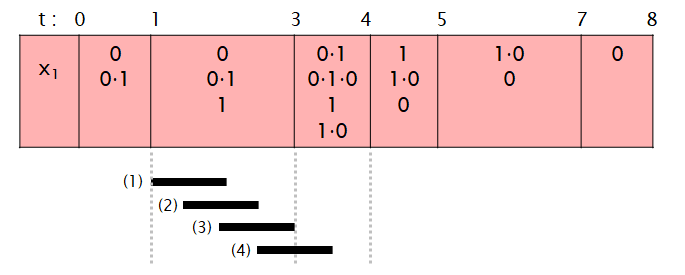
\includegraphics[scale=0.33]{profiles.png}
%	\end{center}
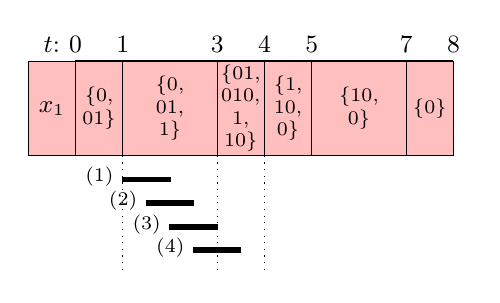
\begin{tikzpicture}[scale=0.6]
	\small
	\draw[thick] (0,-5) -- (8,-5);
	\foreach \x in {0,1,3,4,5,7,8}
	\draw (\x,-5) node[above] {\x};
	\draw (-0.5,-5) node[above] {$t$:};
	
	\draw[fill=pink] (-1,-7) rectangle (0,-5) node[midway] {$x_1$};
	\draw[fill=pink] (0,-7) rectangle (1,-5) node[midway] {\scriptsize\begin{tabular}{c}\{0,\\ 01\}\\\end{tabular}};
	\draw[fill=pink] (1,-7) rectangle (3,-5) node[midway] {\scriptsize\begin{tabular}{c}\{0,\\ 01,\\ 1\}\\\end{tabular}};
	\draw[fill=pink] (3,-7) rectangle (4,-5) node[midway] {\scriptsize{\begin{tabular}{c}\{01,\\ 010,\\ 1,\\ 10\}\\\end{tabular}}};
	\draw[fill=pink] (4,-7) rectangle (5,-5) node[midway] {\scriptsize\begin{tabular}{c}\{1,\\ 10,\\ 0\}\\\end{tabular}};
	\draw[fill=pink] (5,-7) rectangle (7,-5) node[midway] {{\scriptsize\begin{tabular}{c}\{10,\\ 0\}\\\end{tabular}}};
	\draw[fill=pink] (7,-7) rectangle (8,-5) node[midway] {{\scriptsize\begin{tabular}{c}\{0\}\\\end{tabular}}};
	
	\draw[dotted] (1,-7) -- (1,-9.5);
	\draw[dotted] (3,-7) -- (3,-9.5);
	\draw[dotted] (4,-7) -- (4,-9.5);
	
	\draw[fill=black] (1, -7.5 + 0.05) node[left]{{\scriptsize (1)}} rectangle (2, -7.5 - 0.05) ;
	\draw[fill=black] (1.5, -8 + 0.05) node[left] {{\scriptsize (2)}} rectangle (2.5, -8 - 0.05) ;
	\draw[fill=black] (2, -8.5 + 0.05) node[left] {{\scriptsize (3)}} rectangle (3, -8.5 - 0.05);
	\draw[fill=black] (2.5, -9 + 0.05) node[left] {{\scriptsize (4)}} rectangle (3.5, -9 - 0.05);
\end{tikzpicture}
	\caption{The profiles of $J = [0,1)$ with respect to $x_1 \in S$ of \cref{ex:canonseg}. The four representative intervals of each profile is shown with solid black lines below the tabular representation of $\gamma$ for $x_1$.}
	\label{fig:profiles}
	\vspace{-4em}
\end{wrapfigure}

\subsubsection{Computing the Semantics of STL$^+$.}

Putting it all together, given a distributed signal $(S, {\hb})$ and an STL$^+$ formula $\varphi$, we can compute $[(S,{\hb}) \models \varphi]_+$ thanks to the following theorem.

\begin{theorem} \label{cl:algo}
	For every distributed signal $(S,{\hb})$ and STL formula $\varphi$ we have $[(S,{\hb}) \models \varphi]_+ = \top$ (resp. $\bot$, ${\,?}$) iff $\first(\llbracket (S, {\hb}) \models \varphi \rrbracket) = \{1\}$ (resp. $\{0\}$, $\{0,1\}$).
%	\begin{itemize}
	%		\item $[(S,{\hb}) \models \varphi]_{\mathsf{STL}^+} = \top \iff ... = \{1\}$
	%		\item $[(S,{\hb}) \models \varphi]_{\mathsf{STL}^+} = \bot \iff ... = \{0\}$
	%		
	%		\item $[(S,{\hb}) \models \varphi]_{\mathsf{STL}^+} = {\,?} \iff ... = \{0, 1\}$
	%	\end{itemize}
\end{theorem}

%\begin{enumerate}
%	\item 
%	Enumerate the subformulas of $\varphi$ such that each formula has an enumeration number smaller than the numbers of all its subformulas.
%	Let $\varphi_1, \ldots, \varphi_m$ be such an enumeration.
%	Note that $\varphi_1 = \varphi$.
%	
%	\item
%	Compute the canonical segmentation $G_{S} = \{ [t_1, t_2), \ldots, [t_k, t_{k+1}) \}$ of $(S, {\hb})$.
%	
%	\item
%	Compute the value expressions of signals with respect to the canonical segmentation, i.e., for each $1 \leq j \leq k$ and $1 \leq i \leq n$, compute $\gamma([t_j, t_{j+1}), i)$.
%	
%	\item
%	Compute the value expressions of subformulas with respect to the canonical segmentation, i.e., for each $1 \leq j \leq k$ and $1 \leq \ell \leq m$, compute $[S, t_j \models \varphi_\ell]$.
%	
%	\item
%	Output the set $\mathsf{Out}(\varphi, S, {\hb}, \varepsilon, \delta) = \destutter([S,t_1 \models \varphi_1] \cdot \ldots \cdot [S,t_k \models \varphi_1])$ of value expressions. 
%\end{enumerate}


%\small
%\begin{align*}
%	[(S, {\hb}) \models ]_+ &= \first(  )\\
%	[(S, {\hb}) \models AAAAAAAAA]_+ &= \\
%	[(S, {\hb}) \models AAAAAAAAA]_+ &= \\
%	[(S, {\hb}) \models AAAAAAAAA]_+ &= \\
%	[(S, {\hb}) \models AAAAAAAAA]_+ &= \\
%%		\llbracket (S, {\hb}) \models p \rrbracket &= AAAA \\
%%	\llbracket (S, {\hb}) \models \lnot \varphi_1 \rrbracket &= \lnot \llbracket (S, {\hb}) \models \varphi_1 \rrbracket \\
%%	\llbracket (S, {\hb}) \models \varphi_1 \land \varphi_2 \rrbracket &= \llbracket (S, {\hb}) \models \varphi_1 \rrbracket \\
%\end{align*}
%\normalsize
%\SetKwComment{Comment}{/* }{ */}
%\begin{algorithm}
%	\caption{An algorithm with caption}\label{alg:two}
%	\KwData{$n \geq 0$}
%	\KwResult{$y = x^n$}
%	$y \gets 1$\;
%	$X \gets x$\;
%	$N \gets n$\;
%	\While{$N \neq 0$}{
%		\eIf{$N$ is even}{
%			$X \gets X \times X$\;
%			$N \gets \frac{N}{2}$ \Comment*[r]{This is a comment}
%		}{\If{$N$ is odd}{
%				$y \gets y \times X$\;
%				$N \gets N - 1$\;
%			}
%		}
%	}
%\end{algorithm}







\subsubsection{Sets of Boolean Value Expressions as Bit Vectors.}
Evidently, asynchronous products are expensive to compute.
Our implementation of the algorithm we describe in this section relies on the following observation:
Sets of boolean value expressions and their operations can be efficiently implemented through bit vectors.
Intuitively, to represent such a set, we can encode each element using its first bit and its length since value expressions are boolean and always destuttered.
Moreover, to evaluate untimed operations on such sets, we only need to know the maximal lengths of the four possible types of expressions ($0 \ldots 0$, $0 \ldots 1$, $1 \ldots 0$, and $1 \ldots 1$) and whether the set contains $0$ or $1$ (to handle some edge cases).
This is because value expressions corresponding to same segments can be seen as completely asynchronous and the possible interleavings obtained from shorter expressions can be obtained from longer ones.
This approach enables, for example, an algorithm for conjunction of sets of value expressions that runs in $O(|u| + |v|)$ time where $u$ and $v$ are the longest expressions in the two sets.
Note that the same idea also applies to untimed temporal operators.


\subsubsection{Generalization to Real-Valued Signals.}
The methods in \cref{sec:approach} can be extended to real-valued signals and numerical predicates.
The key is that finite-length piecewise-constant signals take finitely many values.
By defining $\Sigma$ as a finite alphabet of these values, we can compute atomic propositions as above.
%Arithmetic operations are handled by computing the asynchronous product of the signals and applying the operation letter-by-letter, transforming the results into atomic propositions via comparison with constants.
For example, if the asynchronous product of two signals $x_1$ and $x_2$ yields $(2\cdot2\cdot3, 1\cdot0\cdot1)$, adding these letter-by-letter results in $3 \cdot 2 \cdot 4$, and comparing with $> 2$ gives $101$. Repeating this for all pairs produces the required atomic proposition.
%\alert{This approach is called \textsc{Orig}.}

We can avoid explicit computation of asynchronous products for some formulas and numerical predicates.
Since signals are asynchronous within segments, we compute potential value sets instead of sequences.
\alert{This approach is called \textsc{Fine}.}
For instance, with $X_1 = \{2,3\}$ and $X_2 = \{0,1\}$, pairwise addition yields $\{2, 3, 4\}$.
Assuming $x_1 + x_2$ is constant within this segment, we can avoid explicit interleaving computations.
While \textsc{Fine} overapproximates traces when order matters, such as in $(x_1 > c_1) \until (x_2 > c_2)$, it preserves precision for formulas like $\LTLalways((x_1 - x_2) \cdot x_3 > c)$.
\alert{The approach \textsc{Coarse}} refines \textsc{Fine} by only considering extreme values, useful for monotonic operations where the extreme values of outputs derive from inputs.
For instance, if $\min X_1 = 2$, $\max X_1 = 3$, $\min X_2 = 0$, and $\max X_2 = 1$, then $\min(x_1 + x_2) = 2$ and $\max(x_1 + x_2) = 4$.
This way, we can efficiently maintain a smaller set of values and still preserve precision for formulas with monotonic operations.
Lastly, assuming the monitor runs on a monitored agent reduces asynchrony by using the agent's clock as a reference point.
\alert{This approach is called \textsc{Relative}.}
We will demonstrate the benefits and downsides of each method in \cref{sec:experiments}.

%\ege{This part is new, please check and maybe try to shorten.}
%The methods described in \cref{sec:approach} and here can be generalized to handle arithmetic operations over real-valued signals and numerical predicates.
%The key observation enabling this is that such finite-length piecewise-constant signals take only finitely many values.
%Then, letting $\Sigma$ be a finite alphabet of these values, we are able to compute the $\gamma$ function as described.
%To handle arithmetic operations, we can compute the asynchronous product of the signals involved and apply the given operation letter-by-letter.
%Finally, to transform them into atomic propositions, we can compare the resulting value expressions letter-by-letter with a constant.
%We call this approach \textsc{Orig}.
%For example, suppose the asynchronous product of two signals $x_1$ and $x_2$ contains $(2\cdot2\cdot3, 1\cdot0\cdot1)$.
%Applying addition to this pair letter by letter would give us $3 \cdot 2 \cdot 4$, and applying the comparison $> 2$ would result in the Boolean value expression $101$.
%Repeating this for all pairs, we obtain the atomic proposition required.
%
%As described in the previous subsection, we can efficiently represent and manipulate Boolean value expressions, avoiding explicit computation of asynchronous products.
%This method does not apply to real-valued signals in general, therefore formulas with numerical predicates cause an additional overhead.
%However, there are several ways how we can avoid explicit computation of asynchronous products for some classes of formulas and numerical predicates.
%
%Since signals are completely asynchronous within segments, we can ignore the order and compute a set of potential \emph{values} instead of a set of \emph{sequences of values}.
%Continuing the example above, instead of repeating the process above for all the interleavings, we can consider the value sets $X_1 = \{2,3\}$ for $x_1$ and $X_2 = \{0,1\}$ for $x_2$ to conclude by pairwise addition that the values of $x_1 + x_2$ come from the set $\{2, 3, 4\}$.
%Then, we can simply assume that $x_1 + x_2$ is constant with one of these values within the segment.  
%We call this approach \textsc{Fine}.
%Notice that ignoring the order may lead to additionally overapproximating the original set of traces.
%Therefore, \textsc{Fine} does not apply to formulas where the order of values matters, e.g.,  $(x_1 > c_1) \until (x_2 > c_2)$.
%Nonetheless, when it applies, e.g. for $\LTLalways((x_1 - x_2) \cdot x_3 > c)$, it saves us the time to explicitly compute the interleavings and the value expressions.
%
%We can take \textsc{Fine} further and only consider the extreme values.
%Some arithmetic operations are \emph{monotonic} in the sense that the extreme values of the output's value expressions can be computed from those of inputs.
%For example, since $\min X_1 = 2$, $\max X_1 = 3$, $\min X_2 = 0$, and $\max X_2 = 1$, we immediately obtain that the minimal and maximal values of $x_1 + x_2$ are 2 and 4.
%This is particularly useful for formulas where the only temporal operator is $\LTLalways$ or $\LTLeventually$.
%We call this approach \textsc{Coarse}.
%
%Finally, instead of assuming that the monitor runs on a separate agent, we can assume it runs on one of the monitored agents.
%This helps reduce the computational overhead caused by asynchrony by taking the agent where the monitor runs as a reference point, removing any uncertainty associated with this agent's signal.
%We call this approach \textsc{Relative}.
%We will demonstrate the benefits and downsides of each of these in \cref{sec:experiments}.